\begin{pa} \label{PA:4.2}
A person walking along a straight path has her velocity in miles per hour at time $t$ given by the function $v(t) = 0.25t^3-1.5t^2+3t+0.25$, for times in the interval $0 \le t \le 2$.  The graph of this function is also given in each of the three diagrams in Figure~\ref{F:4.2.PA1}.
\begin{figure}[h]
\begin{center}
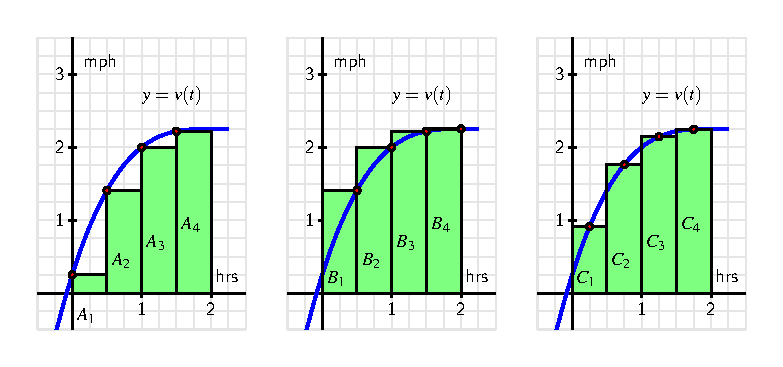
\includegraphics{figures/4_2_PA1.eps}
\end{center}
\caption{Three approaches to estimating the area under $y = v(t)$ on the interval $[0,2]$.} \label{F:4.2.PA1}
\end{figure}
Note that in each diagram, we use four rectangles to estimate the area under $y = v(t)$ on the interval $[0,2]$, but the method by which the four rectangles' respective heights are decided varies among the three individual graphs.
\ba
	\item How are the heights of rectangles in the left-most diagram being chosen?  Explain, and hence determine the value of 
	$$S = A_1 + A_2 + A_3 + A_4$$
	by evaluating the function $y = v(t)$ at appropriately chosen values and observing the width of each rectangle.  Note, for example, that 
	$$A_3 = v(1) \cdot \frac{1}{2} = 2 \cdot \frac{1}{2} = 1.$$
	\item Explain how the heights of rectangles are being chosen in the middle diagram and find the value of
	$$T = B_1 + B_2 + B_3 + B_4.$$
	\item Likewise, determine the pattern of how heights of rectangles are chosen in the right-most diagram and determine
	$$U = C_1 + C_2 + C_3 + C_4.$$
	
	\item Of the estimates $S$, $T$, and $U$, which do you think is the best approximation of $D$, the total distance the person traveled on $[0,2]$?  Why?
\ea
\end{pa} 
\afterpa